\documentclass[11pt]{article} 
\usepackage{deauthor,times,graphicx}
\usepackage{hyperref}
%\usepackage{lineno}
%\linenumbers

% no classified information/data -- only public

\begin{document}

\title{Experiences in exascale scientific data management}

\author{
Mario Lassnig\thanks{E-Mail: Mario.Lassnig@cern.ch}\\CERN \and
Martin Barisits\\CERN \and
Dimitrios Christidis\\UT Arlington
}

\maketitle

\begin{abstract}
Scientific data management has become an increasingly difficult challenge. Modern experiments and instruments are generating unprecedented volumes of data and their accompanying dataflows are becoming more complex. Straightforward approaches are no longer applicable at the required scales and there are few reports on long-term operational experiences. This article reports on our experiences in this field: we illustrate challenges in operating the exascale dataflows of the high energy physics experiment ATLAS, we detail the concepts and architecture of the data management system Rucio that was purposely built to take up these challenges, we describe how other experiments evaluated, modified, and adopted the Rucio system for their own needs, and we show how Rucio will evolve to cope with the ever increasing needs of the community.
\end{abstract}

\section{Introduction}

Many large scale scientific experiments are reaching a breaking point where the growth rate of the collected data greatly exceeds the growth rate of the infrastructure behind them. In the next few years, large instruments similar in scale to the Large Hadron Collider (LHC)~\cite{lhc} and its High-Luminosity upgrade HL-LHC~\cite{hllhc} are coming online, such as the Deep Underground Neutrino Experiment (DUNE)~\cite{dune}, or the Square Kilometre Array (SKA) radio observatory~\cite{ska}. Throughout their lifetimes, these collaborations anticipate massive increases both in the number of data objects they need to handle as well as the total volume of data they need to store. Additionally, increasingly complex computational workflows result in similarly complex dataflows to support them, which can rapidly lead to science-inhibiting complications. Examples include congestion on networks, disorderly space allocations on storage, or erratic transfer schedules. At the same time, there are many smaller communities and experiments who do not want to lose efficient access to the same shared storage and network resources but do not possess a similar level of effort to ensure their sustainability. This brings a variety of challenges to the field of data management as a whole to ensure fair use of all available resources, leading to the need to orchestrate and synchronize dataflows across multiple experiments with potentially competing characteristics.

In this article we address four topics relevant to these challenges: in Section \ref{sec:hep} we describe first-hand experiences developing and operating an exascale data management system for high energy physics, in Section \ref{sec:rucio} we describe the data management system that was used to tackle these challenges, in Section \ref{sec:beyond} we discuss how a diverse set of scientific communities evaluated, modified, and adopted the system for their own needs, and in Section \ref{sec:common} we propose possibilities how to integrate and interconnect widely distributed data management solutions as a cooperating ensemble. We conclude in Section \ref{sec:conc} with a summary and an outlook on future work.

\section{The data challenge in High-Energy Physics}
\label{sec:hep}

The LHC at CERN hosts four major experiments, ATLAS~\cite{atlas}, CMS~\cite{cms}, ALICE~\cite{alice}, and LHCb~\cite{lhcb}. Both ATLAS and CMS are general-purpose particle physics experiments and are designed to exploit the full discovery potential and the huge range of physics opportunities that the LHC provides, whereas ALICE and LHCb focus on detailed precision studies in their respective fields. All experiments are run by large international collaborations. The experiments track and identify particles to investigate a wide range of physics topics, from the study of the Higgs boson~\cite{higgs} to the search for supersymmetry~\cite{susy}, quark-gluon plasma~\cite{plasma}, b-physics~\cite{beauty}, extra dimensions~\cite{extra}, or potential particles that make up dark matter~\cite{darkmatter}.

For the remainder of the article, we will focus on the data management aspects of the ATLAS experiment, as it presents the most diverse dataflow requirements across the LHC experiments. As such, many of the experiences presented are similarly applicable to the other experiments, scaled to their respective experiment sizes. At its current scale, ATLAS is currently managing more than 1 billion files in active use comprising almost 500 Petabytes of data. For scientific integrity and reproducibility, the experiment also needs to keep track of data that has been deleted, which amounts to an additional 1.5 billion historical files. The interaction rate of operations with the data management system are typically beyond 200 Hz and reach up to 500 Hz. This includes diverse operations such as registering new files, searching for data, scheduling old files for deletions, or removing unwanted datasets. The experiment utilizes 120 data centers globally, including 5 supercomputing centers (HPCs), and connects to scientific and commercial cloud storage. There are more than 1000 active users, who in turn require data transfer and deletion rates at 500 Petabytes/year, plus an additional 2.5 Exabytes/year of data access for their ongoing analyses.

\begin{figure}[t]
        \centering
        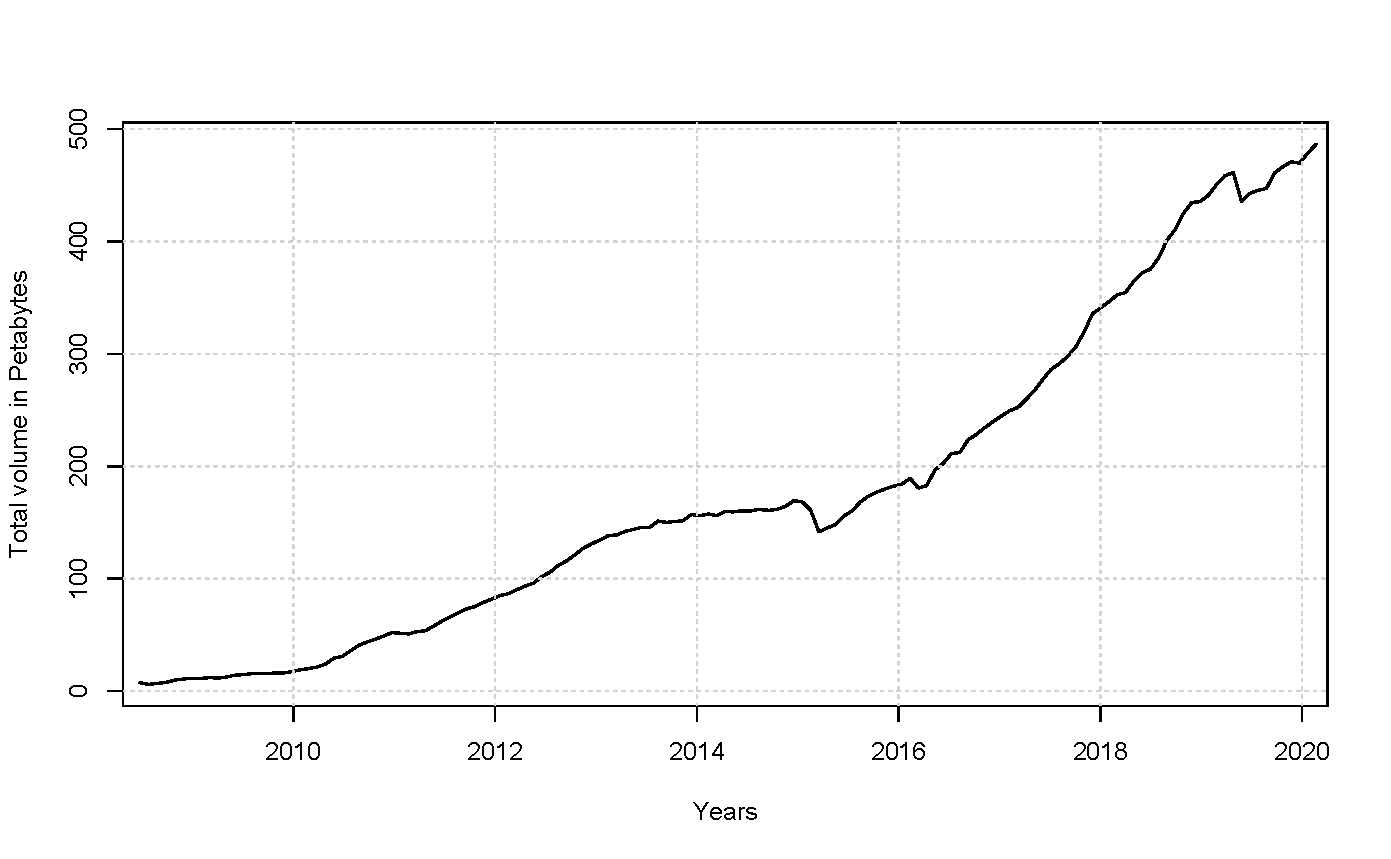
\includegraphics[width=\textwidth]{figs/data_evolution.pdf}
        \caption{The cumulative ATLAS data volume approaches 500 Petabytes in early 2020. Growth has been linear with respect to the scale of the experiment, with considerable data deletion before longer observation periods.}
        \label{fig:atlas_volume}
\end{figure}

Figure \ref{fig:atlas_volume} shows the cumulative data volume from ATLAS starting from 2008, when the distributed computing infrastructure was commissioned. The data growth in high energy physics is not exponential, rather there are linear growth intervals at varying intensities. It can be seen that the data growth of LHC Run 1 from April 2011 until September 2012 is distinctively higher than the following LHC shutdown period until April 2015, during which only simulation data was produced. The first major deletion campaign to free up space on the available storage marks the beginning of the four-year-long LHC Run 2. The vastly increased data rate after 2015 reflects the higher intensity of the LHC. Notably, the growth rate of the simulated data also increased, which required a second major deletion campaign at the beginning of the current LHC shutdown period. We anticipate a similar deletion campaign in late 2020 before the start of LHC Run 3.

\begin{figure}[t]
        \centering
        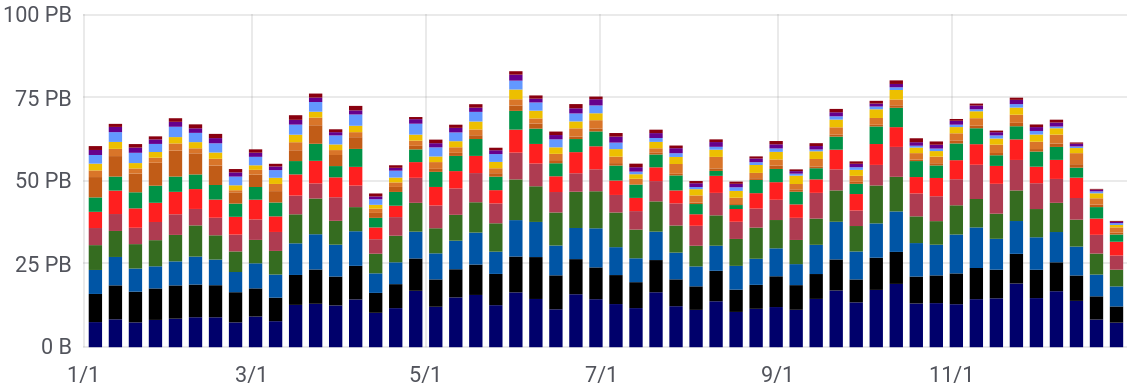
\includegraphics[width=\textwidth]{figs/ATLAS_Flow.png}
        \caption{ATLAS data transfers and downloads are regularly above 50 Petabytes per week throughout 2019. The prominent dip during the festive season is due to CERN closure. Colors indicate geographical regions.}
        \label{fig:atlas_transfer_rate}
\end{figure}

Figure \ref{fig:atlas_transfer_rate} shows the weekly ATLAS data transfers and downloads. The transfers between data centers are enacted whenever required by the computational workflow, and the downloads subsequently occur from the storage to the node which does the actual computation. Users downloading data directly to their workstations accounts for roughly 12 percent of the overall download volume. The colors indicate the 12 geographical regions of the experiment, out of which 4 larger regions are responsible for half of the total capacity. The global weekly transfer volume is typically more than 50 Petabytes, but can burst significantly above 70 Petabytes. There is a prominent dip at the end of the year which corresponds to the two-week closure of the CERN facilities during the festive season. The number of files transferred per week is typically beyond 50 million. The number of file deletions is equivalent to roughly 10 Petabytes per week, arising from the needs of the embarrassingly parallel computational workflow, which results in many temporary intermediate files. The number of files deleted per week is typically more than 20 million. In terms of transfer failures, the typical rate is more than 4 million failures per week, mostly due to faulty hardware such as broken disks or electrical problems. Deletion failures are typically rarer, below 1 million per week, mostly due to the implementation of the WebDAV-based deletion protocol in the storage systems. Scheduled deletion of files which were already removed from storage do not count as failures. Major deletion failures occur rarely, on the order of once per quarter, which typically points to hardware failures at a data center with massive data loss. One of the major successes of the ATLAS data management system is that it can handle a large variety of these failures transparently, that is recover and restore data from alternative, pristine sources to ensure global data safety.

\begin{figure}[t]
        \centering
        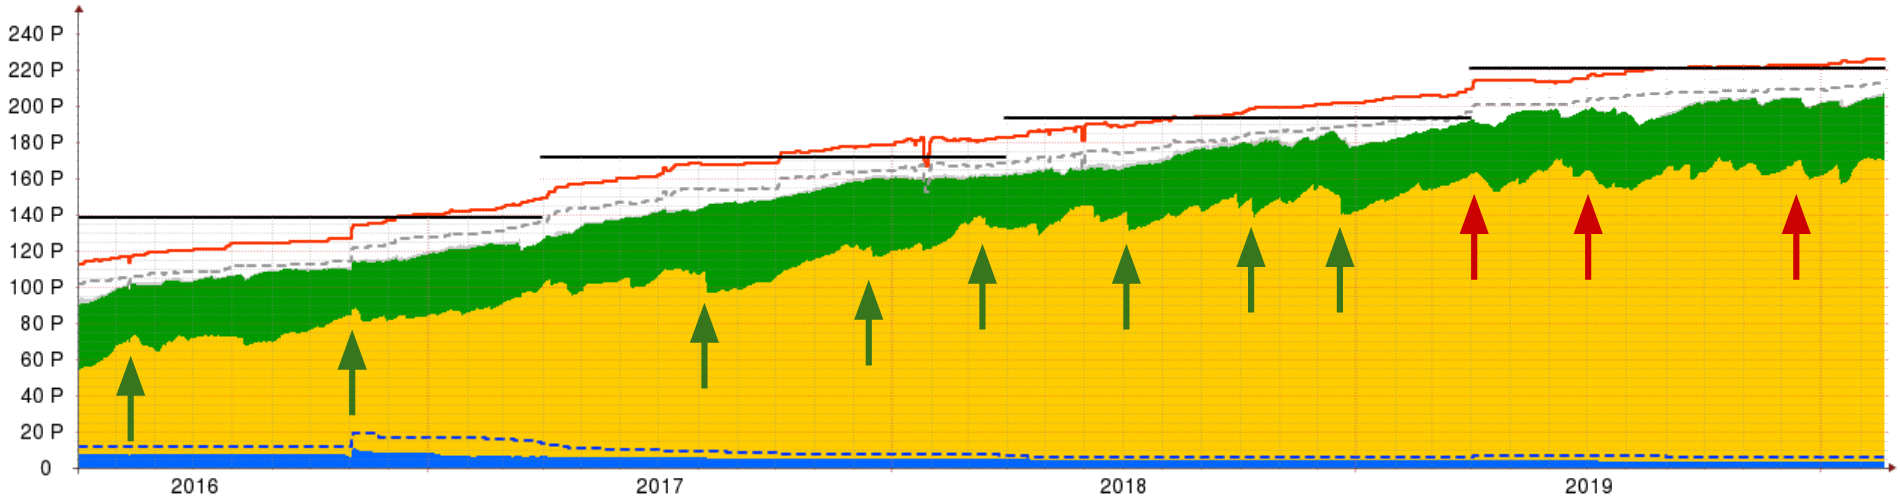
\includegraphics[width=\textwidth]{figs/lifetime_model.png}
        \caption{The green and red arrows indicate the application of the lifetime model for scheduled deletion of unused data on pledged disk resources in ATLAS. Green arrows are rule-based deletion, red arrows are file-based deletion. Black lines indicate data center pledges, the red line actual available storage. The yellow data volume indicates primary data, the green data volume is cached data.}
        \label{fig:lifetime_model}
\end{figure}

We now highlight three examples from data management operations in ATLAS, which help to achieve the experiment's needs: the data lifetime model~\cite{lifetime}, sliding window processing~\cite{carousel}, and data recovery~\cite{rucio}. As the first example, the lifetime model works as follows. If left unchecked, the creation of new data within the experiment would quickly exhaust all available storage space. Members of the operations team, together with other groups from the collaboration, need to spend considerable effort to identify and delete datasets that are no longer needed, mostly via consensus across scientific groups. Multiple procedures have been developed over the years to alleviate this, however the most prominent and effective is the lifetime model. Within ATLAS, each dataset is annotated with a wide variety of metadata. Policies are defined based on these metadata that dictate when they are expected to expire. For example, raw data coming out of the ATLAS detector are kept forever, whereas data in analysis object formats are kept for two years and log files are kept for only one year. These policies allow for the lifetime of the dataset to be further extended based on the last access date, which is based on a distributed data access tracing system. This allows the deletion of data to be postponed beyond its expected lifetime as long as it is in constant use. The lifetime model itself does not however initiate the deletion of the expired datasets. Instead, a procedure is set where an announcement is made which datasets are scheduled for expiry, and users are given a period to submit exception requests. These requests are reviewed by the operations team, and the final selection is then scheduled for deletion. Applications of the lifetime model are shown in Figure~\ref{fig:lifetime_model}, indicated by the green and red arrows. Typically multiple iterations are necessary per year to keep enough storage space available for distributed processing given the available storage capacity of the data center. Originally, only rules enforcing dataset distribution would be removed, that is the files themselves would remain as cached copies on storage and would be deleted only when the data center they were stored at was running out of space. In late 2018, the execution of the lifetime model was adjusted such that the rules were removed and that the files were immediately purged. The reason for this was to reduce the latency between the deletion requests and the space being made available for new data. This can be seen by the gradual decrease of the yellow primary data volume, with no correlating increase of the green cached data volume.

\begin{figure}[t]
    \centering
    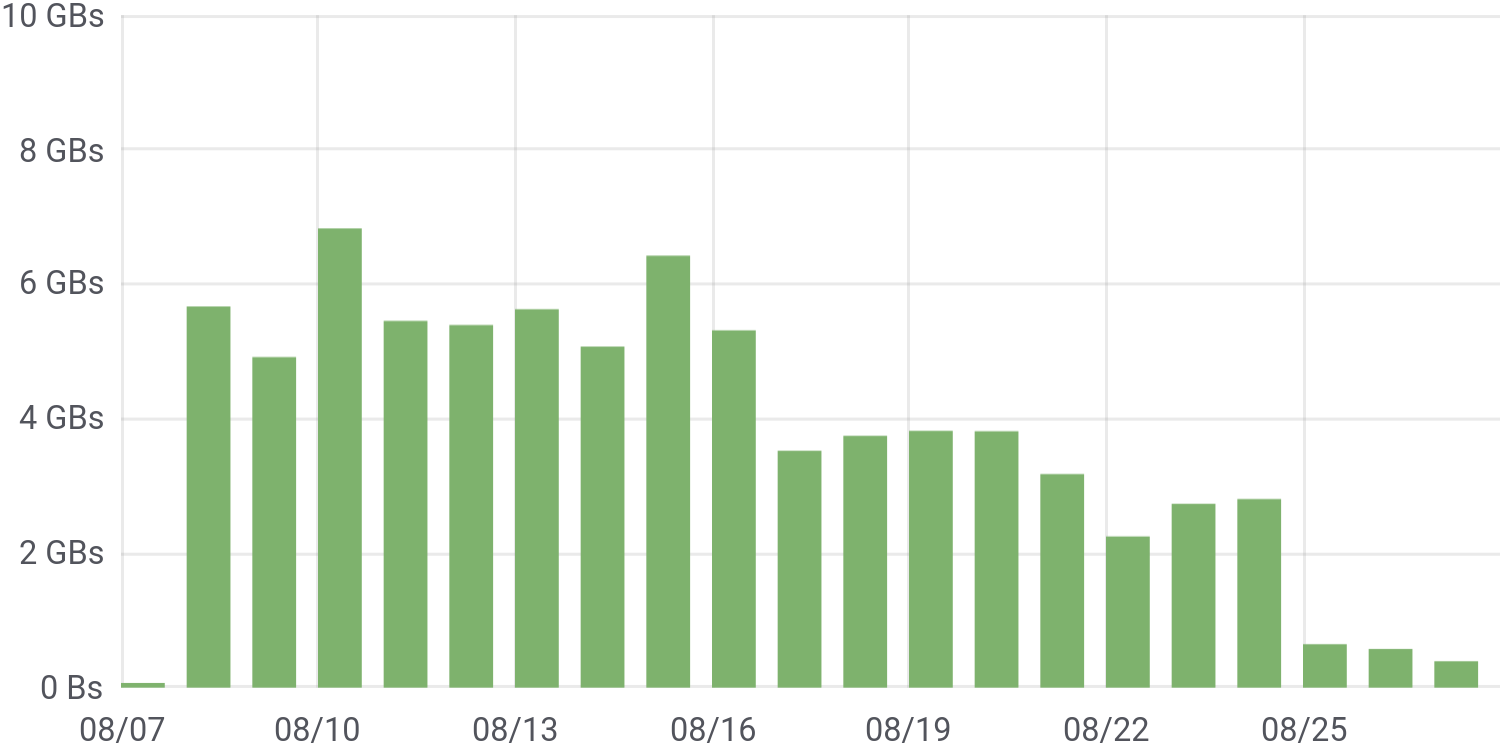
\includegraphics[width=0.49\linewidth]{figs/data_carousel_2019.png}
    \hfill
    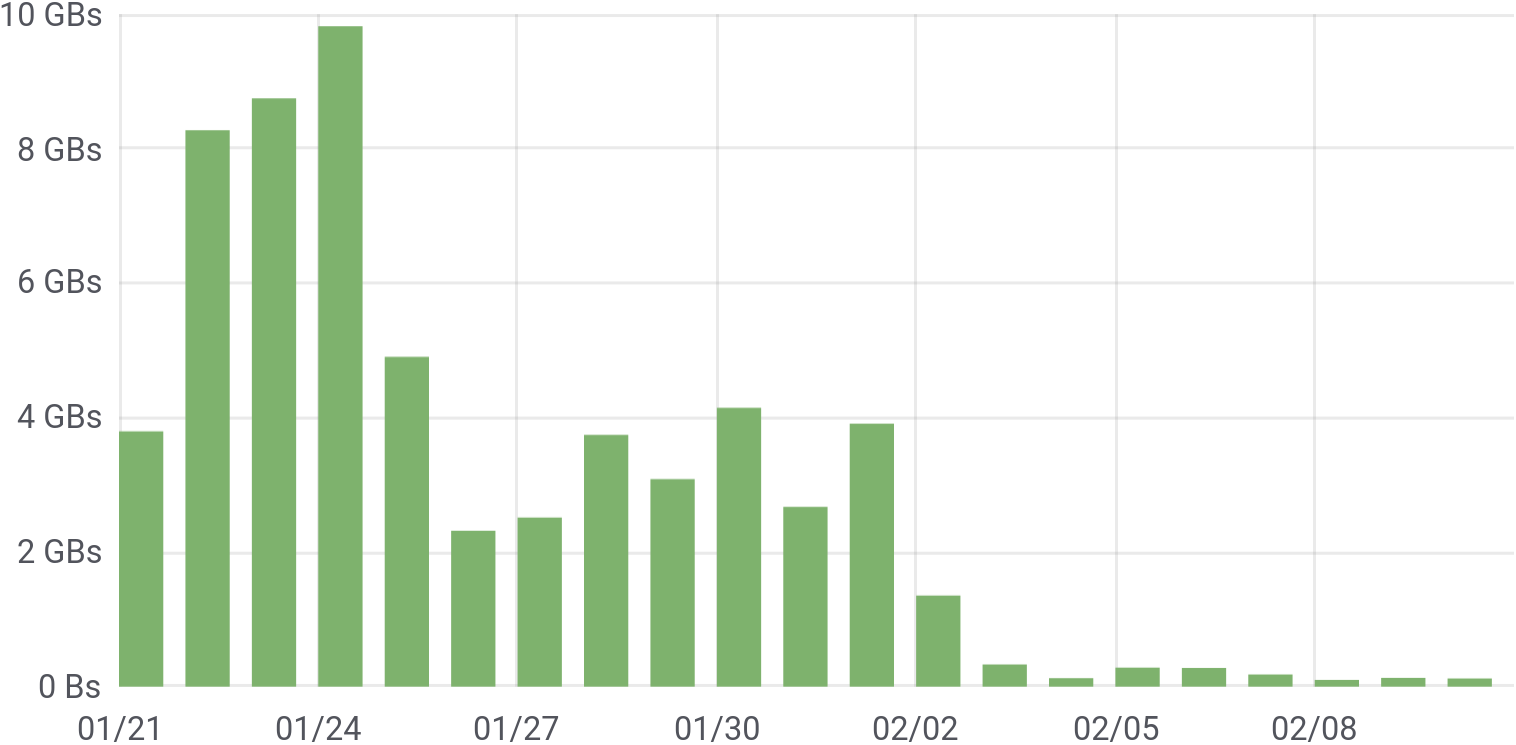
\includegraphics[width=0.49\linewidth]{figs/data_carousel_2020.png}
    \caption{Data Carousel tape recall rate. On the left, measurements from the 2019 exercise with slow ramp-up and 5 GB/s throughput. On the right, the 2020 exercise with fast ramp-up and doubling of throughput.}
    \label{fig:data_carousel}
\end{figure}

The second example is the sliding window process, internally called the Data Carousel. In ATLAS, typical processing workflows meant recalling all necessary data from tape onto disk, and then starting the processing. These recalls might take from many days up to several weeks but were necessary to ensure constant high CPU utilization. With recent advances in the workflow management system and data management system, a new processing method was developed which allows the use of a sliding window process to ensure only data necessary for a particular step in the processing was recalled while still maintaining high CPU utilization. The main benefit is in the cost reduction for data centers, because instead of purchasing expensive disk-based storage a large fraction of funding can now be shifted to tape with a significantly lower cost per byte ratio. Figure \ref{fig:data_carousel} shows the improvements in the process from 2019 to 2020. On the left hand side, the first iteration of the process showed a significant ramp-up time of more than one day before stabilizing at 5 MBps. This functional test demonstrated that the process is feasible but required significant improvements in terms of throughput performance. During the next months, several strategies were developed, including tuning of the tape systems by the data centers, latency reduction in communication, and most importantly the exploitation of the dataset namespace to schedule the tape-writing and their recalls in groups beneficial to the computation. As seen on the right hand side, these improvements caused immediate ramp-up and a doubling of throughput capacity. At the time of writing, the process is now in use in production by ATLAS and has already been used in a significant reprocessing campaign. In this campaign, which involves the processing of 5.7 Petabytes of data, never more than 1 Petabyte is resident on disk and several hundred Terabytes are processed and removed in daily cycles.

The third example is the data recovery process. Given the number of files registered in the data management system and the number of ongoing transfers, data corruption or loss is unavoidable. The reasons can vary from corrupted network packets to faulty disk and tape drives, or even natural disasters, such as flooding of data centers. The data management system is flexible and easily allows multiple file replicas to be stored in different countries and on different storage media. For the long-term archival of raw data, experience has shown that maintaining two copies on tape storage in two different locations, one of which is at CERN, is sufficient. Each file registered in the system has a defined checksum, typically Adler-32. The reason for using Adler-32 is the algorithm's performance and cumulative property, which allows in-flight calculation. The checksum is propagated to the transfer mechanism so that if a file is corrupted, either at the source or the destination, then the transfer will immediately fail. These transfer failures can occur for a variety of different reasons, so pattern matching is applied to the error message to provide an indication where corruption occurs. Should the source file appear to be corrupted, then the replica is marked as suspicious. The data management interface collects and lists these suspicious replicas and providers a simple mechanism for operators to declare them lost. If there are other replicas of a file then a transfer will be automatically scheduled to recover it. The process is partially automated: if a file has multiple transfer failures and more than one replica, then it will be automatically declared as lost. The data management system provides configurable thresholds to fine-tune this process. The patterns themselves are also configurable. The same treatment also applies to missing files: the mechanism can trigger the files to be declared as suspicious and potentially lost. However, automated consistency checks are also conducted as a proactive measure, using periodic extracts from the data management system catalog. These are compared against periodic extracts from the storage systems in the data centers. If a file exists in the former but is missing from the latter, then it is marked as suspicious. If a file exists in the latter but not in the former, then it is marked as dark data, which means it is occupying space without being able to be used by the experiment. The data management system ensures that such files are deleted from the data centers. This is a crucial process, which aims to prevent the accumulation of non-addressable data and in turn loss of available storage space.

\section{The Rucio system for scientific data management}
\label{sec:rucio}

\begin{figure}[t]
        \centering
        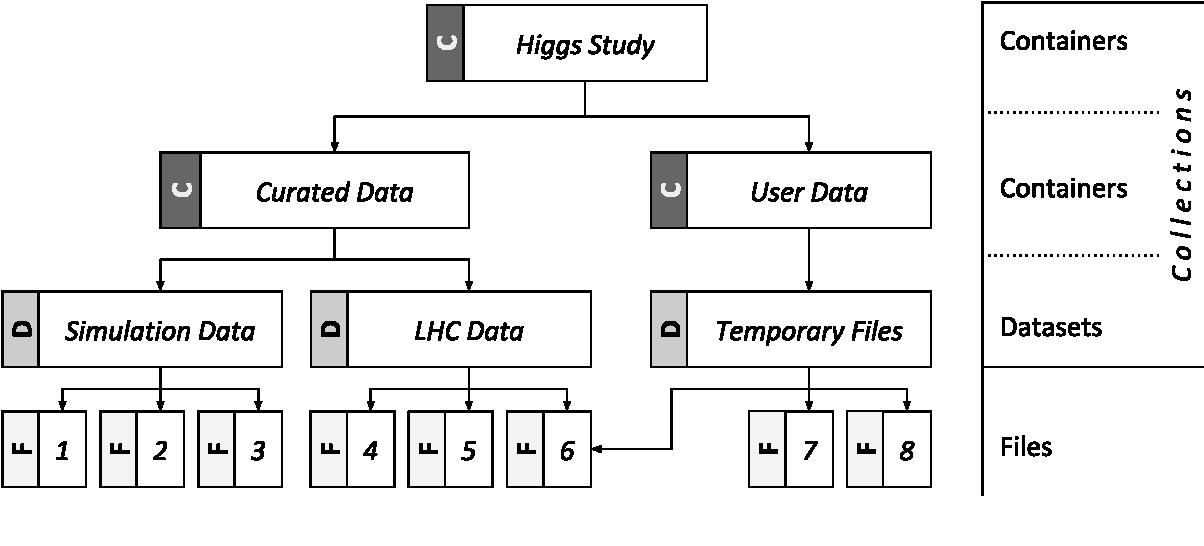
\includegraphics[width=\textwidth]{figs/rucio_namespace.pdf}
        \caption{The namespace is organized via dynamic collections of three different types, called {\em Data Identifiers (DIDs)}: containers, datasets, and files. Only datasets can contain files, but files can be in multiple datasets. All operations can be enacted on all DIDs, regardless the type, and are respectively resolved.}
        \label{fig:rucio_namespace}
\end{figure}

\begin{figure}[t]
        \centering
        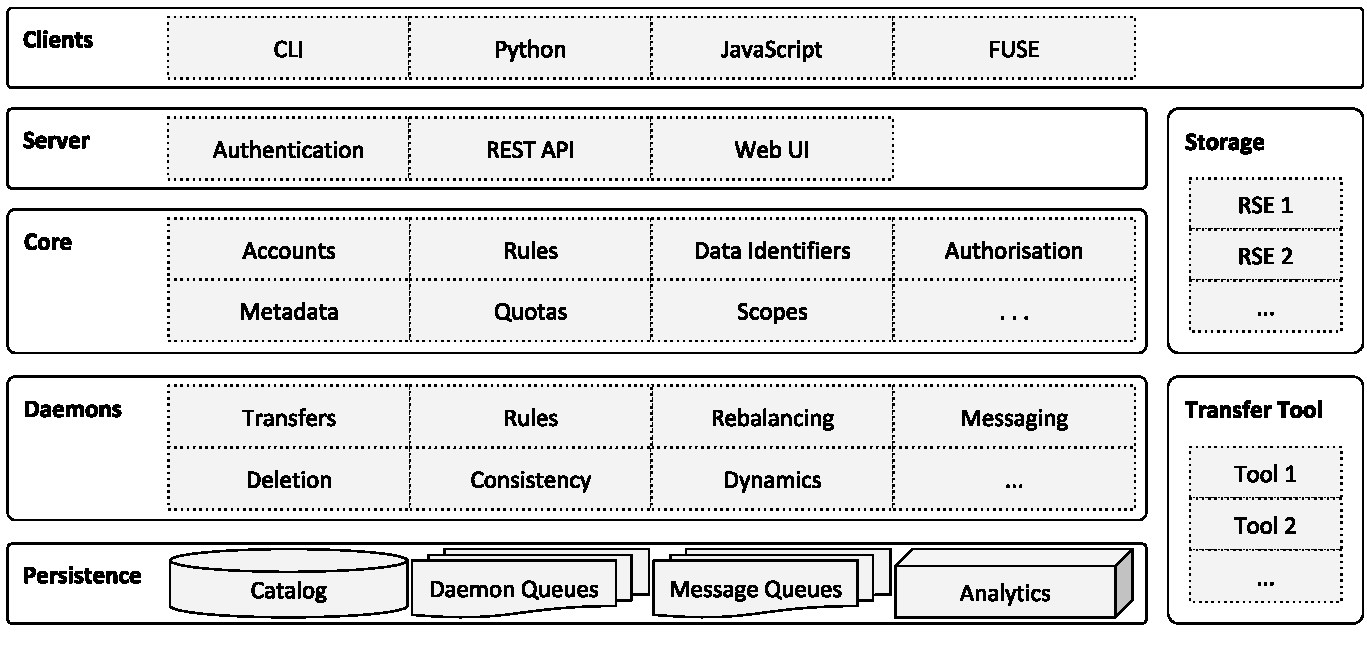
\includegraphics[width=\textwidth]{figs/rucio_arch.pdf}
        \caption{Rucio is loosely-coupled, with its catalog and state persisted in a transactional database. Daemons coordinate their work in shared queues, external systems are notified via message queues, and analytics storage is kept separately. The storage and and transfer tools are modular and integrated vertically across the layers.}
        \label{fig:rucio_arch}
\end{figure}

The ATLAS experiment has developed the Rucio system to handle all its distributed data needs. An extensive summary article describes Rucio in great detail~\cite{rucio}, therefore we only give an overview here.

Rucio manages location-aware data in a heterogeneous distributed environment, including creation, location, transfer, deletion, and annotation. Declarative orchestration of dataflows with both low-level and high-level policies is the main mode of operation. The software is free and open-source, licensed under Apache v2.0, and makes use of established open-source toolchains. In terms of functionality, Rucio provides a mature and modular scientific data management federation, including seamless integration of scientific and commercial storage and their corresponding network systems. Data is stored in files, but can contain any potential payload. The storage facilities can be distributed at multiple locations belonging to different administrative domains, which makes it particularly useful for large collaborations. It was designed following more than a decade of operational experience in large-scale data management~\cite{dq} and has dataflow automation as its guiding principle.

Rucio is organized in a scoped namespace of Data Identifiers (DIDs). DIDs are unique and can be files or collections. Collections can be datasets which then contain files, or containers which consist of other containers and datasets. Figure \ref{fig:rucio_namespace} shows an example namespace of several DIDs, notably the possibility to have overlapping contents across collections. Datasets and containers are logical units which usually share some scientific context, for example, files with results from a specific study, or data taken in during a specific interval. These collections also enable the user to execute certain bulk operations such as transfers or downloads in a convenient way, as Rucio correctly interprets operations on DIDs depending on their type.

The logical representation of storage in Rucio is called a Rucio Storage Element (RSE). An RSE is a description of network-accessible storage with certain attributes, such as hostname, port, protocols and priorities. An RSE is only a logical abstraction of storage space, there is no need to run any Rucio software at a data center. Simply providing the RSE configuration to Rucio is sufficient and thus allows to federate a wide variety of heterogeneous storage systems. Interaction with the physical storage is orchestrated via the published protocols, for example gsiftp, WebDAV, root, S3, and many more. Thus RSEs can be any type of storage, typically disk or tape systems, scientific and commercial cloud providers, or even supercomputers. The physical representations of files on storage are called replicas. A replica is always associated to a specific RSE. Files can have one, or many replicas depending on the policies and access patterns of the organization. Files without replicas are marked as deleted and are kept in the historical namespace for reference. The orchestration of dataflows in Rucio is done via a descriptive concept called replication rules. These rules define policies on DIDs to ensure that a certain number of replicas are made available on RSEs matching a defined policy for a certain amount of time. Thus replication rules serve the purpose of transferring data to an RSE but also to protect the data from deletion until the lifetime of the rule expires.

The Rucio architecture, as shown in Figure \ref{fig:rucio_arch}, is based on a distributed design split into a multiple layers, each with their own set of components: the clients, server, core, daemons, and persistence layer. While details of this architecture are discussed in the summary article it is noteworthy that the architecture is fully horizontally scalable while at the same time responsive to the required work. The system can thus be used from single data center deployments up to globally distributed federations. Starting from the most basic data cataloging requirements, more advanced features can be activated selectively depending on the needs of the experiment. For example, the system supports dynamic schema-free and schema-based metadata collection and queries, data transfers between heterogeneous facilities, diverse authentication and authorization mechanisms, web user interfaces, API and CLI integrations, extensive monitoring of dataflows, and expressive high-level and low-level data policy engines. As previously mentioned, automatic data corruption identification and recovery is one of the most appreciated features of the system.

\section{Establishing a community}
\label{sec:beyond}

As the scientific community has become more aware of the success of Rucio within ATLAS, several experiments asked if it would be possible to evaluate and potentially adopt the system for their needs. This section distills the reports from a variety of sciences from the corresponding article~\cite{beyond}.

The first scientific experiment adopting Rucio as a data management system was the AMS-02~\cite{ams} collaboration. AMS is a particle detector attached to the International Space Station measuring antimatter in cosmic rays. There are many scientific goals of AMS, but one of the major objectives is the search for evidence of dark matter. The Rucio system was installed and managed by the Taiwanese Academy of Science (ASGC). This was done in collaboration and support of the core Rucio team at CERN. ASGC team members spent many weeks at CERN to learn from the direct operational experience of Rucio at CERN and to work together with the developers to adapt the system to scientific usecases beyond high energy physics. During this collaboration multiple features were added to the Rucio code base and the ASGC team developed a powerful web interface extension serving their local community. The Rucio system at ASGC is now in use not only for AMS, but a variety of smaller experiments hosted at their institute.

The XENON dark matter experiment~\cite{xenondm} is operated in the underground research facility Laboratory National del Gran Sasso (LNGS) in Italy. It is aiming to directly detect weakly interacting massive particles (WIMPs). The first stage are raw data, which are distributed with Rucio among grid computing facilities within the European Grid Infrastructure (EGI) and the Open Science Grid (OSG) in the US, including SDSC's Comet Supercomputer and the HPC campus resources. Second and third stage are processed data which are kept at the Research Computing Center (RCC) in Chicago, which is also its main data analysis center. XENON1T has taken 800+ TB of raw data and ran multiple re-processing campaigns for improving data quality in ongoing data analysis tasks~\cite{xenoncp}. The upcoming XENONnT upgrade will take 1 Petabyte per year. Processing and Monte Carlo simulation campaigns are planned at the major infrastructures of EGI and OSG. A newly developed tool integrates Rucio in the XENONnT data flow and data product locations are registered. All data products will be distributed within Rucio to the connected grid computing facilities for storage. Tape storage will be integrated in Rucio this time and dedicated grid locations are reserved to store the raw data product. XENONnT is the first hard Python3 dependency on Rucio. For analysts, the RCC in Chicago is again the main data analysis centre and provides user access to high level data products at a nearby location. Analysts can also define and produce own data products for analysis purposes outside the run database or grid storage at any time. 

CMS performed an evaluation of data management systems from early 2018 through summer 2018, and eventually selected Rucio. The plan is to have Rucio deployed and ready for LHC Run 3: The transition period will last from 2018-2020, and the CMS team has expressed excitement about participating in a sustainable community project. The production infrastructure is based on Docker, Kubernetes, Helm, and OpenStack, with the official Rucio Helm charts customized with minimal configuration changes for CMS. The zero-to-operating cluster timing including dependencies is in the order of tens of minutes which allows fast and easy integration with CMS software and infrastructure; Rucio upgrades are nearly instantaneous. This also allows CMS to have its production and Rucio testbed on a shared set of resources. The developer's environment is identical to various flavors of central clusters, which makes integration easy. In 2019, the first full-fledged test distributed 1 million files between all CMS T1 and T2 data centers. The critical factor for data management scalability is the number of files, not the actual volume of data to be moved. The entire successful test took 1.5 days, and was purely driven by dataset injection rate. It ran in parallel to regular experiment activity.

The Deep Underground Neutrino Experiment (DUNE) is a neutrino experiment under construction, comprising a near detector at Fermilab and a far detector at the Sanford Underground Research Facility (SURF) that will observe neutrinos produced at Fermilab. DUNE's data management challenges are unique because they have multiple geographically separated detectors asynchronously collecting data, at an expected rate of tens of Petabytes per year. DUNE is also sensitive to supernovae, which potentially produce hundreds of Terabytes over a 100 second period. It is a large collaboration that intends to store and process data at many data centers worldwide, and the current ProtoDUNE prototype detector has already recorded 6 Petabytes of reconstructed data. The next test beam run for both single and dual phase prototypes is expected in 2021-22. DUNE has a Rucio instance at Fermilab with a PostgreSQL backend, and has contributed several database extensions to Rucio. So far, 1+ million files have been cataloged from ProtoDUNE, including raw and reconstructed data. Rucio is being used to distribute ProtoDUNE data from CERN and FNAL to other data centers for analysts. The replication rules make this easy; making a rule for a dataset and data center or group of data centers eliminates operational overhead for DUNE. The current integration plan is to progressively replace the legacy data management system, and transition to a purely Rucio based solution. The main challenge is that DUNE intends to make significant use of HPC resources, and the data management system needs to integrate with many very heterogeneous supercomputing data centers. This is in line with the global HEP move towards using more HPC resources. Additionally DUNE data will benefit from fine grained object store style access, however it is not clear how to combine this with the traditional file based approach. The DUNE community has expressed that they are interested to contribute to these developments in the near future.

The Square Kilometre Array (SKA) is an intergovernmental radio telescope project to be built in Australia and South Africa. With receiving stations extending out to a distance of more than 3'000 kilometers from a concentrated central core, it will allow astronomers to create the most sensitive images of the Universe. The SKA Regional Centers will provide a platform for transparent data access, data distribution, post-processing, archive storage, and software development. Up to 1 Petabyte will be ingested from each telescope, and made available for access and post-processing around the globe. SKA will therefore need a way to manage data in a federated way across many physical data centers transparent to the user. SKA has begun evaluating Rucio for SRC data management. Data has been uploaded, replicated, and deleted from storage systems using custom replication rules and sustained data transfers have already been demonstrated from South Africa to the United Kingdom. A full mesh functional test has been put in place and is demonstrating connectivity. Tests were conducted using data from the LOFAR telescope, an SKA pathfinder instrument. Currently, the Elasticsearch/Logstash/Kibana (ELK) monitoring stack~\cite{elk} is being set up up, and already 8M data operation events over more than one year of testing have been ingested. The evaluation experience using Rucio has been positive and is now formalized through the H2020 ESCAPE project, the European Science Cluster for Astronomy and Particle Physics ESFRI research infrastructures~\cite{escape}. The main findings from the test include the arduous need for X.509 certificates across storage systems, which is now being addressed via alternatives such as token-based authentication and authorization. In addition, an in-depth look at the ELK monitoring and dashboards will be performed to see where they still need to be extended. Another major point is the integration with the DIRAC~\cite{dirac} workflow management system, matching the Belle II experiment needs, for a full end-to-end use case. Another use case will be similar to LHC Tier-0 processing with event-driven data management and processing. The inclusion of Australian storage for long-distance tests with a focus on network optimization is also upcoming.

The Laser Interferometer Gravitational-Wave (LIGO) Observatory~\cite{ligo}, based in the US, is a large-scale observatory to detect cosmic gravitational waves and to develop gravitational-wave observations as an astronomical tool. Virgo~\cite{virgo} is the European equivalent interferometer, based in Italy at the European Gravitational Observatory (EGO). LIGO and Virgo are building the International Gravitational Wave Network (IGWN), with a combined 20 Terabytes of astrophysical strain data and 1 Petabyte of raw data per instrument per observing year. A data management solution is needed for offline deep searches and parameter estimation, as well as support for dedicated and opportunistic resources, as well as archival data. Rucio now enhances the IGWN data management through a large choice of protocols, an accessible catalog, comprehensive monitoring and support for detector data flows. This includes domain-specific daemons that register new dataframes in the Rucio catalog and then create rules to trivially implement dataflow to the archives and resources. IGWN has stated that they will investigate many opportunities beyond this, as well as being happy to update to a modern, high-availability version of existing functionality. Rucio is now being used in production for limited frame data replication to volunteering data centers, and a transition away from LDR is expected over the coming months. Upcoming work includes integration of existing data discovery services and remote data access, for example, enhanced database redundancy, and management of new data products, for example, analysis pipeline data products. A mountable Rucio POSIX namespace is under development as an alternative for gravitational wave software distribution.

The Belle II experiment~\cite{belleii} is a particle physics experiment designed to study the properties of B mesons. The data requirements include 70 storage systems with around 200 Petabytes of data expected by the end of data-taking, with 2 replicas distributed over 6 data centers. Physics data taking started in 2019. Belle II's current distributed data management uses a bespoke design with adequate performance and supports up to 150'000 transfers/day. Some scalability issues in the system were addressed, but others are inherent to the design of the data management system, most importantly the lack of automation: this means that data distribution and deletion are done by experts at a very fine granularity. The Belle II team at Brookhaven National Laboratory (BNL) are evaluating Rucio as an alternative and all studies so far look promising. Most importantly, the performance on the PostgreSQL database at BNL shows capabilities beyond the Belle II requirements. Integration of Rucio with the rest of the Belle II distributed computing system, based on DIRAC, is planned in two stages. In the first stage the current data management APIs are replaced with an implementation that uses Rucio under the hood. This is mostly transparent to the rest of Belle II and allows bi-directional transition between the two implementations. However, this still relies on a legacy file catalog, and does not take full advantage of Rucio and its functionalities, being limited to the current APIs by definition. Nevertheless this stage allows the BNL team to gain experience in a production environment of using the DIRAC WFMS with Rucio. The second stage integration leads to an eventual migration that will use Rucio as the master file catalog, using a new DIRAC plugin to remove the dependency on the legacy file catalog.

\section{Towards a common approach }
\label{sec:common}

During the evaluation together with these communities, Rucio has established a fully community-driven development process. Requirements and issues are publicly discussed via weekly development meetings, on GitHub~\cite{ruciogithub}, and group messaging based on Slack~\cite{rucioslack}. The project also hosts a yearly community workshop for developers and users to meet and to discuss the evolution of the software stack. The core development team provides guidance on design, architecture, as well as tests, and integration and evolves the development environment and continuous integration framework. Whereas packaging and high-level release planning is done by members of the core development team, the development is largely driven by contributors from the community. Contributions are reviewed by both the community as well as the core development team. Recent improvements in containerization and testing frameworks have significantly lowered the barrier to entry for newcomers. However, while contributing to the project has gotten simpler the project is specifically looking for maintained feature developments, thus sustainability is an important factor discussed with every contribution. One interesting aspect is that communities have started to help each other without the involvement of the core team, leading to a self-sustaining process that has been effective across time zones due to multi-continent involvement.

Although recent developments with containers and Kubernetes has made the deployment of Rucio very simple, the operation and maintenance of a data management system is still a significant effort for smaller scientific communities, which very often operate with very little personpower but still have significant data requirements. The UK Science and Technology Facilities Council (STFC) has been developing an enhancement to offer a data management service for multiple communities based on a single Rucio instance. This feature enables one Rucio instance to be virtually partitioned to serve multiple organizations, thus enabling communities to benefit from Rucio services while keeping the operational footprint low.

The need for operational cooperation has been acknowledged by many experiments, and a cross-experiment Operational Intelligence~\cite{opint} effort has been started. Thousands of tickets are filed in the issue tracking system per year, which have to be followed by the operations teams of the various systems. In the context of Rucio, this effort seeks to exploit the wealth of dataflow traces to increase the level of automation. The first proposed models apply to the prediction of intelligent data placements and access patterns, time-series analyses to estimate of the time needed to complete transfers, or anomaly detection techniques to predict network failures. Recording and analyzing operator actions can be used to automate tasks and to suggest possible solutions to repeated issues.

Another oft-requested feature from the data centers was support for cloud storage to allow more dynamic possibilities for capacity increases. This was developed within the Data Ocean project~\cite{dataocean}, which was an R\&D effort between ATLAS and Google. The idea of the project was to enable ATLAS to explore the use of different computing models by using Google resources, to allow ATLAS users to benefit from the Google infrastructure, and at the same time give Google real science use cases to improve their cloud platform. The project has been highly successful and follow-up developments enhanced the Rucio interfaces to be cloud provider agnostic. Now Rucio can serve as an enabler for scientific experiments who want transparent access to a multitude of diverse cloud storage providers.

\begin{figure}[t]
    \centering
    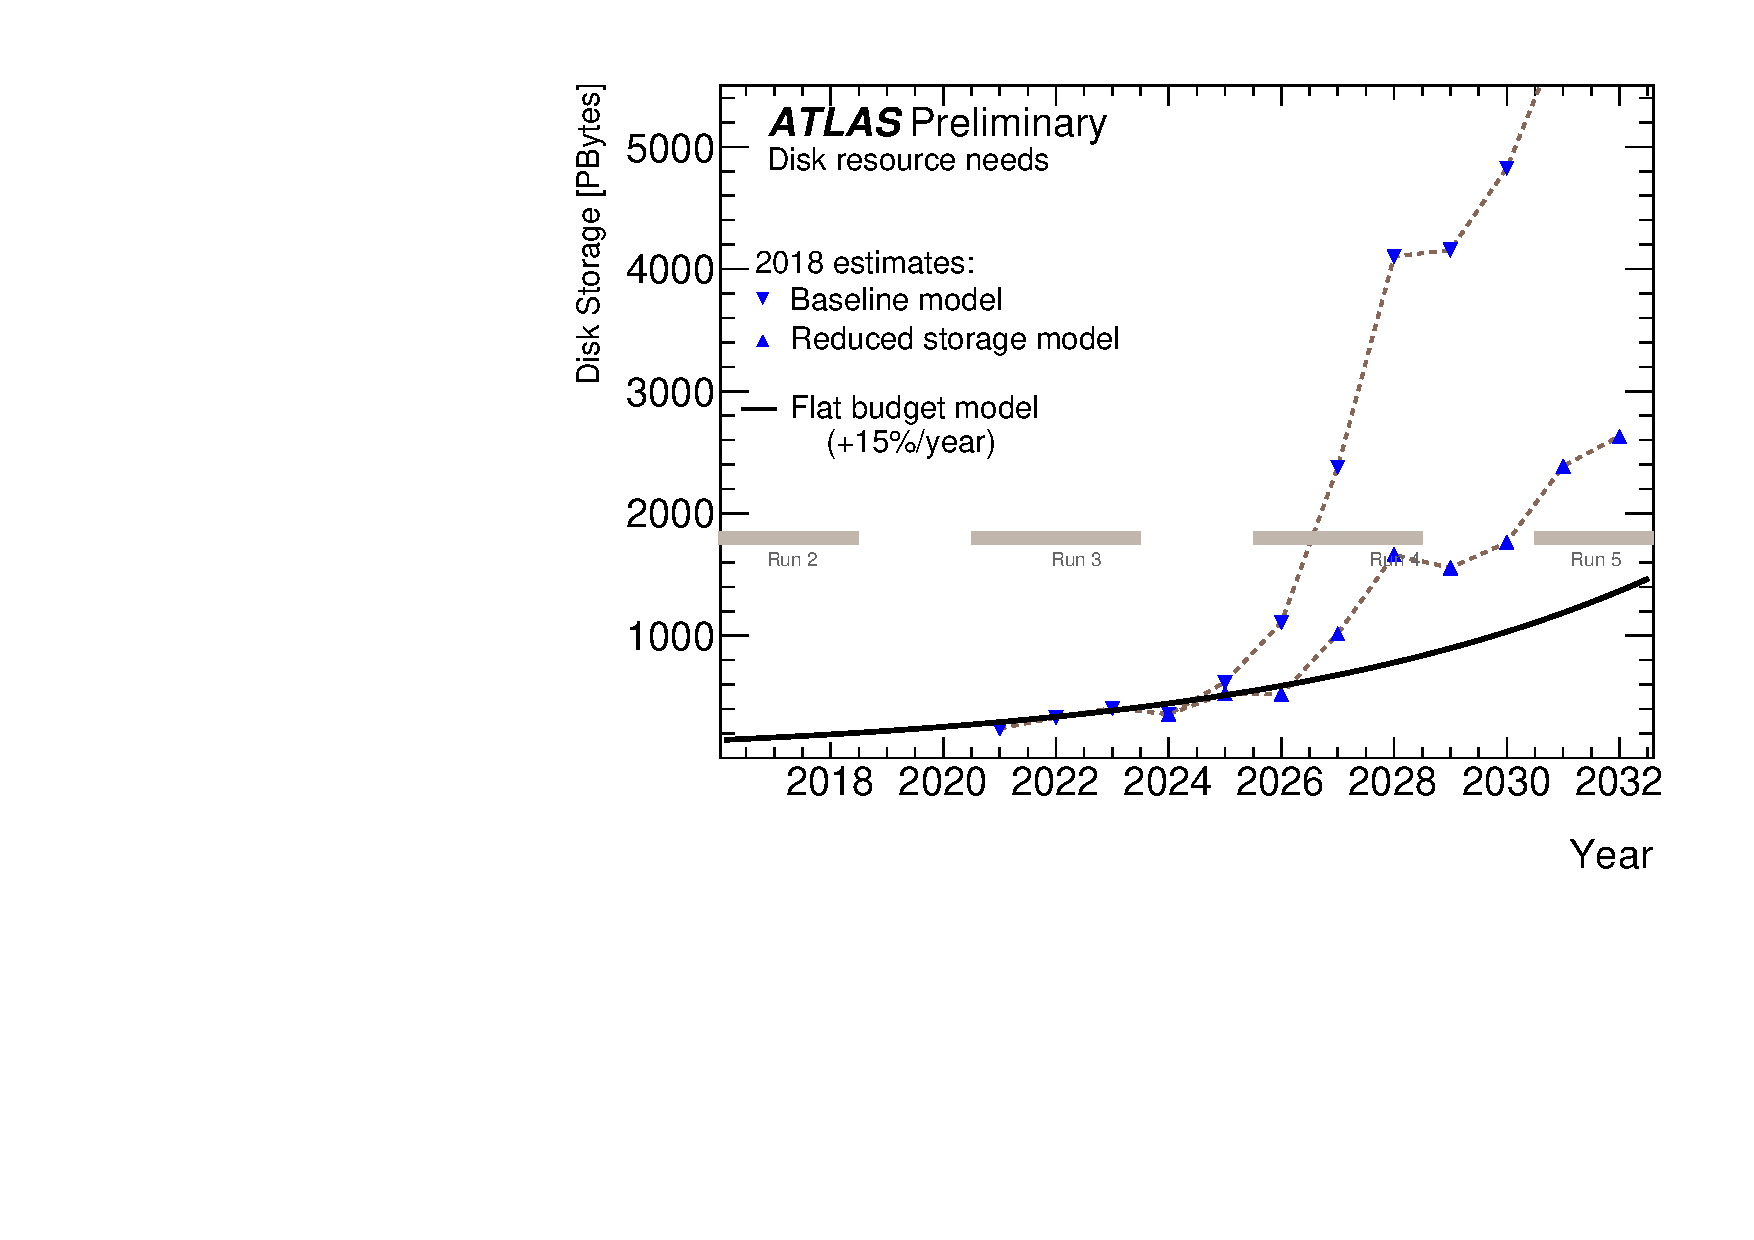
\includegraphics[width=0.49\linewidth]{figs/atlas.pdf}
    \hfill
    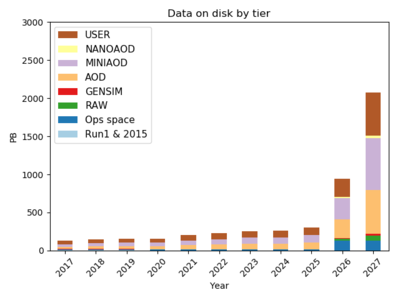
\includegraphics[width=0.49\linewidth]{figs/cms.png}
    \caption{On the left, the estimated total disk resources from ATLAS in Petabytes needed for the years 2018 to 2032. On the right, the equivalent plot from CMS for the years 2017 to 2027. The expected data rates from HL-LHC will exceed funding capabilities even with reduced storage models after 2026.}
    \label{fig:hllhc}
\end{figure}

Finally, the two major topics in scientific data management in the next years are the immediate growth rates of single experiments, and the resulting contention across experiment infrastructures on a limited set of shared storage and network resources. As shown in Figure \ref{fig:hllhc} for ATLAS and CMS, the data growth at the HL-LHC beyond 2026 is significantly above any potential infrastructure growth. Therefore, the high energy physics community has prepared a white paper~\cite{roadmap} to lay out the plans to tackle this challenge. At its core, it employs multiple strategies for data organization, management and access (DOMA)~\cite{doma} that include mechanisms such as analysis model changes, dynamic use of storage quality of service, transparent distributed caching, network flow control using SDNs, and much more. Many of these strategies rely on having Rucio as a common data management system, with the objective to help steer dataflows across multiple experiments as a cooperating ensemble. The development of the exchange of dataflow state as well as cross-experiment namespace and scheduling will be crucial.

\section{Conclusions}
\label{sec:conc}

The LHC data needs have been driving a variety of data management developments for more than two decades. Throughout many attempts, the collected experiences led to the development of the Rucio system, which has proven flexible, efficient, and robust. The openness of the system, the autonomous declarative way of handling dataflows, the transparent handling of data incidents, and the capability to monitor the flows in detail have all contributed the success of Rucio. Many communities have now joined and are actively contributing. In conclusion, Rucio is a successful collaborative open source project that is rapidly developing into a common standard for scientific data management.

\section*{Acknowledgments}

This work has been done as part of distributed computing research and development programs across many collaborating institutes, organizations, agencies, and communities.  We thank all our colleagues for their support.

\begin{thebibliography}{99}
\itemsep=1pt
\begin{small}

\bibitem{lhc}
L.~Evans and P.~Bryant.
\newblock LHC Machine.
\newblock JINST 3:0 S08001, 2008.
\newblock \url{https://doi.org/10.1088/1748-0221/3/08/S08001}{https://doi.org/10.1088/1748-0221/3/08/S08001}

\bibitem{hllhc}
G.~Apollinari, O.~Brüning, T.~Nakamoto and L.~Rossi.
\newblock High Luminosity Large Hadron Collider HL-LHC.
\newblock CERN Yellow Rep.\  (2015) no.5,  1.
\newblock \url{https://doi.org/10.5170/CERN-2015-005.1}{https://doi.org/10.5170/CERN-2015-005.1}

\bibitem{dune}
R.~Acciarri et~al.
\newblock Long-Baseline Neutrino Facility (LBNF) and Deep Underground Neutrino Experiment (DUNE).
\newblock 2016.
\newblock \url{https://arxiv.org/abs/arXiv:1601.05471}{https://arxiv.org/abs/arXiv:1601.05471}

\bibitem{ska}
A.~Chrysostomou, R.~Bolton, G.~R.~Davis.
\newblock The Square Kilometre Array: Challenges of distributed operations and big data rates.
\newblock Proc.\ Observatory Operations: Strategies, Processes, and Systems VII; Volume 10704:1070419 (2018).
\newblock \url{https://doi.org/10.1117/12.2309554}{https://doi.org/10.1117/12.2309554}

\bibitem{atlas}
ATLAS Collaboration.
\newblock The ATLAS Experiment at the CERN Large Hadron Collider.
\newblock JINST, 3:0 S08003, 2008.
\newblock \url{https://doi.org/10.1088/1748-0221/3/08/S08003}{https://doi.org/10.1088/1748-0221/3/08/S08003}

\bibitem{cms}
CMS Collaboration.
\newblock The CMS Experiment at the CERN LHC.
\newblock JINST, 3:0 S08004, 2008.
\newblock \url{https://doi.org/10.1088/1748-0221/3/08/S08004}{https://doi.org/10.1088/1748-0221/3/08/S08004}

\bibitem{alice}
ALICE Collaboration.
\newblock The ALICE experiment at the CERN LHC.
\newblock JINST, 3:0 S08002, 2008.
\newblock \url{https://doi.org/10.1088/1748-0221/3/08/S08002}{https://doi.org/10.1088/1748-0221/3/08/S08002}

\bibitem{lhcb}
LHCb Collaboration.
\newblock The LHCb Detector at the LHC.
\newblock JINST, 3:0 S08005, 2008.
\newblock \url{https://doi.org/10.1088/1748-0221/3/08/S08005}{https://doi.org/10.1088/1748-0221/3/08/S08005}

\bibitem{higgs}
ATLAS and CMS Collaborations.
\newblock Combined measurement of the Higgs boson mass in pp collisions at $\sqrt{s}$=7 and 8 {TeV} with the ATLAS and CMS experiments.
\newblock Phys.Rev.Lett., 114:0 191803, 2015.
\newblock \url{https://doi.org/10.1103/PhysRevLett.114.191803}{https://doi.org/10.1103/PhysRevLett.114.191803}

\bibitem{susy}
ATLAS Collaboration.
\newblock Summary of the ATLAS Experiment's sensitivity to supersymmetry after LHC Run 1 - interpreted in the phenomenological MSSM.
\newblock JHEP, 1510:0 134, 2015.
\newblock \url{https://doi.org/10.1007/JHEP10(2015)134}{https://doi.org/10.1007/JHEP10(2015)134}

\bibitem{plasma}
P.~Braun-Munzinger and J.~Stachel.
\newblock The quest for the quark-gluon plasma.
\newblock Nature 448 (2007), 302-309.
\newblock \url{https://doi.org/10.1038/nature06080}{https://doi.org/10.1038/nature06080}

\bibitem{beauty}
M.~Pepe Altarelli and F.~Teubert.
\newblock $B$ Physics at LHCb.
\newblock Int.J.Mod.Phys A23 (2008), 5117-5136.
\newblock \url{https://doi.org/10.1142/S0217751X08042791}{https://doi.org/10.1142/S0217751X08042791}

\bibitem{extra}
ATLAS Collaboration.
\newblock Search for TeV-scale gravity signatures in high-mass final states with leptons and jets with the ATLAS detector at $\sqrt{s}=13$ TeV.
\newblock Phys.Lett. B, 760:0 520--537, 2016.
\newblock \url{https://doi.org/10.1016/j.physletb.2016.07.030}{https://doi.org/10.1016/j.physletb.2016.07.030}

\bibitem{darkmatter}
ATLAS Collaboration.
\newblock Constraints on mediator-based dark matter and scalar dark energy models using $\sqrt{s} = 13$ TeV $pp$ collisions at the LHC with the ATLAS detector.
\newblock ATLAS-CONF, 051, 2018.
\newblock \url{https://inspirehep.net/record/1702555}{https://inspirehep.net/record/1702555}

\bibitem{lifetime}
A.~Filipčič.
\newblock ATLAS Distributed Computing Experience and Performance During the LHC Run-2.
\newblock J.Phys.Conf.Ser. 898(5):052015.
\newblock \url{https://doi.org/10.1088/1742-6596/898/5/052015}{https://doi.org/10.1088/1742-6596/898/5/052015}

\bibitem{carousel}
X.~Zhao, A.~Klimentov et al.
\newblock ATLAS Data Carousel.
\newblock Submitted to EPJ Web.Conf. (2020).
\newblock \url{https://indico.cern.ch/event/773049/contributions/3474425/}{https://indico.cern.ch/event/773049/contributions/3474425}

\bibitem{rucio}
M.~Barisits, T.~Beermann, F.~Berghaus et~al.
\newblock Rucio: Scientific Data Management.
\newblock Comput Softw Big Sci (2019) 3:11.
\newblock \url{https://doi.org/10.1007/s41781-019-0026-3}{https://doi.org/10.1007/s41781-019-0026-3}

\bibitem{dq}
M.~Branco et al.
\newblock Managing ATLAS data on a petabyte-scale with DQ2.
\newblock J.Phys.Conf.Ser. 119 (2008) 062017.
\newblock \url{https://doi.org/10.1088/1742-6596/119/6/062017}{https://doi.org/10.1088/1742-6596/119/6/062017}

\bibitem{beyond}
M.Lassnig et al.
Rucio beyond ATLAS: Experiences from Belle II, CMS, DUNE, EISCAT3D, LIGO/VIRGO, SKA, XENON.
\newblock Submitted to EPJ Web.Conf. (2020).
\newblock \url{https://indico.cern.ch/event/773049/contributions/3474416/attachments/1937611/3211761/Rucio_CHEP19.pdf}{https://indico.cern.ch/event/773049/contributions/3474416}

\bibitem{ams}
AMS-02 RICH Collaboration.
\newblock The AMS-02 RICH detector: Status and physics results.
\newblock Nucl.Instrum.Meth. A952 (2020) 161797.
\newblock \url{https://doi.org/10.1016/j.nima.2019.01.024}{https://doi.org/10.1016/j.nima.2019.01.024}

\bibitem{xenondm}
E.~Aprile et al.
\newblock Dark Matter Search Results from a One Ton-Year Exposure of XENON1T.
\newblock Phys.Rev.Lett. 121 2018 111302.
\newblock \url{https://doi.org/10.1103/PhysRevLett.121.111302}{https://doi.org/10.1103/PhysRevLett.121.111302}

\bibitem{xenoncp}
D.~Ahlin et al.
\newblock The XENON1T Data Distribution and Processing Scheme.
\newblock EPJ Web Conf. 214 2019 03015.
\newblock \url{https://doi.org/10.1051/epjconf/201921403015}{https://doi.org/10.1051/epjconf/201921403015}

\bibitem{elk}
O.~Andreassen, C.~Charrondière and A.~De Dios Fuente.
\newblock Monitoring Mixed-Language Applications with Elastic Search, Logstash and Kibana (ELK).
\newblock \url{https://doi.org/10.18429/JACoW-ICALEPCS2015-WEPGF041}{https://doi.org/10.18429/JACoW-ICALEPCS2015-WEPGF041}

\bibitem{escape}
ESCAPE - European Science Cluster of Astronomy \& Particle physics ESFRI research infrastructures.
\newblock H2020-INFRAEOSC-2018-2.
\newblock Grant agreement ID: 824064.
\newblock \url{https://projectescape.eu}{https://projectescape.eu}

\bibitem{dirac}
F.~Stagni et al.
\newblock DIRAC in Large Particle Physics Experiments.
\newblock  J.Phys.Conf.Ser. 898 (2017) no.9, 092020.
\newblock \url{https://doi:10.1088/1742-6596/898/9/092020}{https://doi:10.1088/1742-6596/898/9/092020}

\bibitem{ligo}
J.~Aasi et al.
\newblock Advanced LIGO.
\newblock Class. Quantum Grav. 32, 074001 (2015).
\newblock \url{https://doi.org/10.1088/0264-9381/32/7/074001}{https://doi.org/10.1088/0264-9381/32/7/074001}

\bibitem{virgo}
F.~Acernese et al.
\newblock Advanced Virgo Status.
\newblock J. Phys. Conf. Ser. 1342 (2020) no.1,  012010.
\newblock \url{https://doi.org/10.1051/epjconf/201818202003}{https://doi.org/10.1051/epjconf/201818202003}

\bibitem{belleii}
T.~Kuhr.
\newblock Belle II at the Start of Data Taking.
\newblock EPJ Web Conf. 214 (2019) 09004.
\newblock \url{https://doi.org/10.1051/epjconf/201921409004}{https://doi.org/10.1051/epjconf/201921409004}

\bibitem{ruciogithub}
Rucio Repository
\newblock \url{https://github.com/rucio/rucio}{https://github.com/rucio/rucio}

\bibitem{rucioslack}
Rucio Team Slack
\newblock \url{https://rucio.slack.com}{https://rucio.slack.com}

\bibitem{opint}
ATLAS and CMS Collaborations.
\newblock Operational Intelligence.
\newblock Submitted to EPJ Web.Conf. (2020).
\newblock \url{https://indico.cern.ch/event/773049/contributions/3473362/attachments/1937928/3212143/CHEP_2019_Operational_Intelligence_-_rev05.pdf}{https://indico.cern.ch/event/773049/contributions/3473362}

\bibitem{dataocean}
ATLAS Collaboration.
\newblock The Data Ocean Project: An ATLAS and Google R\&D collaboration.
\newblock EPJ Web Conf. 214 (2019) 04020.
\newblock \url{https://doi.org/10.1051/epjconf/201921404020}{https://doi.org/10.1051/epjconf/201921404020}

\bibitem{roadmap}
HEP Software Foundation Collaboration.
\newblock A Roadmap for HEP Software and Computing R\&D for the 2020s.
\newblock Comput.Softw.Big Sci. 3 (2019) no.1, 7
\newblock \url{https://doi.org/10.1007/s41781-018-0018-8}{https://doi.org/10.1007/s41781-018-0018-8}

\bibitem{doma}
D.~Berzano et al.
\newblock Data Organization, Management and Access (DOMA)
\newblock White Paper.
\newblock \url{http://arxiv.org/abs/arXiv:1812.00761}{http://arxiv.org/abs/arXiv:1812.00761}

\end{small}
\end{thebibliography} 

\end{document}


